\documentclass[../ZF_Wing.tex]{subfiles}

\begin{document}


\paragraph{Einfache Buchhaltung}
\begin{itemize}
	\item Einnahmen und Ausgaben nach Datum sortiert
	\begin{itemize}
		\item Lediglich festgehalten, dass Geld eingonemmen oder ausgegeben wurde
	\end{itemize}
\end{itemize}


\paragraph{Doppelte Buchhaltung}
\begin{itemize}
	\item Auf welchem Konto Bewegung stattfand
	\item Wozu das Geld verwendet wurde
\end{itemize}


\subsection{Überblick Rechnungswesen}
\begin{figure}[H]
\centering
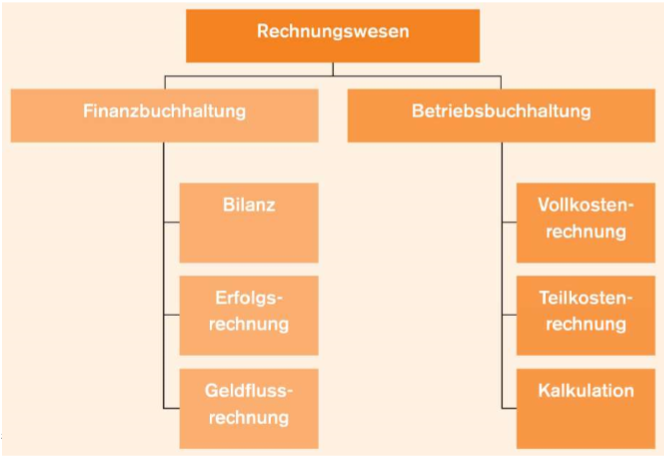
\includegraphics[width=0.3\textwidth]{Resources/Image/Rechnungswesen.png}
\caption{\label{fig:Rechnungswesen}Rechnungswesen.}
\end{figure}

\subsection{Jahresabschluss: Bilanz und Erfolgsrechnung}

\begin{multicols}{2}

\begin{itemize}
	\item Aktiv und Passivbestände am Anfang und am Schluss einer Rechnungsperiode
	\item Momentaufnahme - bezieht sich auf einen Zeitpunkt
	\item \textcolor {teal} {\textbf{Vermögen}}
\end{itemize}
\begin{table} [H]

\begin{tabular}{l|l}
\textbf{Bilanz}\\
\hline
\colorbox{pink!30}{\textbf{(a)} }

\\\hline
&\colorbox{pink!30}{\textbf{(p)} }\\
\hline
& Gewinn\\
\hline

\end{tabular}
\end{table}

\columnbreak


\begin{itemize}
	\item Aufwände und Erträge in einem Zeitraum
	\item \textcolor {teal} {\textbf{Finanzierung des Vermögens}}
\end{itemize}

\begin{table} [H]
\begin{tabular}{l|l}
\textbf{Erfolgsrechnung}\\
\hline
\colorbox{pink!30}{\textbf{A)} }
\\\hline
Gewinn \\
\hline
&\colorbox{pink!30}{\textbf{(E)} }\\
\hline
\end{tabular}
\end{table}

\end{multicols}

\subsubsection{Gegenüberstellung von Aktiven und Passiven}

\begin{figure}[H]
\centering
\includegraphics[width=0.3\textwidth]{Resources/Image/Gegenüberstellung.png}
\caption{\label{fig:Gegenüberstellung}Gegenüberstellung.}
\end{figure}

\subsubsection{Funktion der Bilanz}

\begin{table} [H]
\begin{tabular}{l|l}
\colorbox{orange!30} {\textbf{Funktion}} & \colorbox{orange!30} {\textbf{Erklärung}}\\
\hline
\textbf{Dokumentation} & Bestandesaufnahme der vorhandenen Vermögen  \\
& und Schulden an einem Stichtag\\
\hline
\textbf{Gewinnermittlung} & Gewinn bzw. Verlust einer bestimmten \\
& Periode ersichtlich\\
\hline
\textbf{Information} & Intern \\
&(als Steuerungsinstrument für das Unternehemen)\\
& sowie extern(Kapitalgeber, Statt usw.) über\\ &finanzielle Lage des Unternehmens\\
\end{tabular}

\end{table}

\subsubsection{Aktiven}
\begin{table} [H]
\begin{tabular}{l|l|l}
\colorbox{orange!30} {\textbf{Gliederung}} & \colorbox{orange!30} {\textbf{Erklärung}}\\& & \colorbox{orange!30} {\textbf{Typische Konti}}\\
\hline
\textbf{Umlaufvermögen} & -Abwicklung operativen Geschäfts \\
& - Innerhalb eines Jahres liquidierbar \\
&& - flüssige Mittel (Kasse, Post-und Bankguthaben)\\
&& - Debitoren(GH bei Kunden)\\
&& - Vorräte \\
\hline
\textbf{Anlagevermögen} & Nicht zur kurzfristigen Veräusserungen bestimmt \\
&& - Finanzanlagen\\
&&(Aktien, Obligationen usw.)\\
&& - Mobile Sachanlagen\\&& (Maschinen,Fahrzeuge,Einrichtungen)\\
&& - Immobile Sachanlagen (Liegenschaften)\\
&& - Immaterielle Anlagen\\
&&(Patente, Marken,Goodwill)\\
\hline
\end{tabular}

\end{table}


\subsubsection{Passiven}
\begin{table} [H]
\begin{tabular}{l|l|l}
\colorbox{orange!30} {\textbf{Gliederung}} & \colorbox{orange!30} {\textbf{Erläuterung}}\\& & \colorbox{orange!30} {\textbf{Typische Konti}}\\
\hline
\textbf{Fremdkapital} & - befristet bzw. Kündbar \\
& - FK-geber nicht am Unternehmen beteiligt \\
& - FK-geber nicht am Unternehmen beteiligt\\
& - FK-geber hat kein Mitspracherecht und haftet nicht \\
& - FK-geber nicht am Unternehmen beteiligt \\
& - kurzfristiges FK (bis 1Jahr)\\
& - langfristiges FK (mehr als 1 Jahr) \\
&& - Kreditoren (Schulden bei Lieferanten)\\
&& - Darlehen \\
&& - Hypothek \\
&& - Rückstellungen \\
\hline
\textbf{Eigenkapital} & Schuld Unternehmens gegenüber Eigentümern \\
&& - Kapital (EK, Aktienkapital)\\
&& - Reserven\\
&& - Gewinn(Gewinnvortrag, Jahresgewinn)\\
\hline
\end{tabular}

\end{table}

\subsection{Erfolgsrechnung: Gegenüberstellung von Aufwand und Ertrag}
\begin{table}[H]
\begin{tabular}{l|l}
\textbf{Aufwand} & \textbf{Ertrag} \\
\hline
Betriebsaufwand & Betriebsertrag\\
\hline
Betriebsfremder Aufwand & Betriebsfremder Ertrag\\
\hline
Ausserordentlicher Aufwand & Ausserordentlicher Ertrag\\
\hline
\colorbox {blue!10}{\textbf{Rein-/Nettogewinn}} \\
\hline
\end{tabular}
\end{table}

\subsubsection{Erfolgsrechnung}
\begin{table}[H]
\begin{tabular}{l|l|l}
\colorbox{orange!30} {\textbf{Gliederung}} & \colorbox{orange!30} {\textbf{Erklärung}}\\& & \colorbox{orange!30} {\textbf{Typische Konti}}\\
\hline
\textbf{Aufwände} & - Wofür Unternehmen wie viel Geld ausgegeben hat \\
& - wie stark Vermögenswerte verbraucht wurden\\
&& - Materialaufwand/Warenaufwand\\
&& - Personalaufwand \\
&& - Betriebsaufwand(Mietaufwand,\\
&&  Verwaltungsaufwand, Werbeaufwand,\\
&&  Abschreibungen usw.)\\
&& - Übriger Aufwand\\


\hline
\textbf{Erträge} & - Wofür Unternehmen wie viel Geld eingenommen hat \\
& - wie stark Vermögenswerte gewachsen sind\\
&& - Produktion-/Handels-/\\
&& Dienstleisungsertrag\\
&& - Übriger Ertrag \\
\end{tabular}
\end{table}


\subsubsection{Gliederung der Erfolgsrechnung}
\begin{figure}[H]
\centering
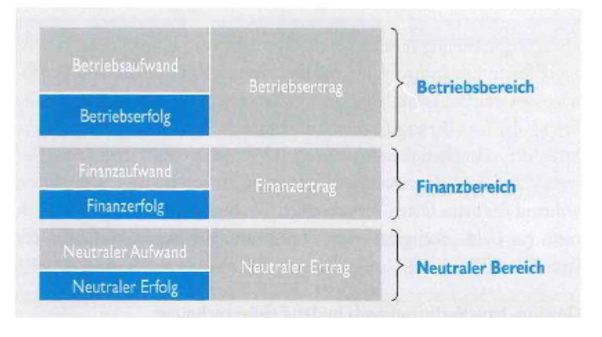
\includegraphics[width=0.3\textwidth]{Resources/Image/GliederungER.png}
\caption{\label{fig:GliederungER}GliederungER.}
\end{figure}

\subsubsection{Erfolgsrechnung: Ausweis verschiedener Gewinngrössen}
\begin{figure}[H]
\centering
\includegraphics[width=0.3\textwidth]{Resources/Image/Gewinngrössen.png}
\caption{\label{fig:Gewinngrössen}Gewinngrössen.}
\end{figure}

\subsection{Geldflussrechnung}
\begin{table}[H]
\begin{tabular}{l|l}
\colorbox{orange!30} {\textbf{Geldflussbereiche}} & \colorbox{orange!30} {\textbf{Erklärung}}\\
\hline
\textbf{Geschäftsbereich} & - alle liquiditätswirksamen Einnahmen und Ausgaben durch Geschäftstätigkeit\\
& - Einnahmen höher als Ausgaben = Cashflow\\
& - Ausgaben höher als Einnahmen = Cashloss\\
\hline
\textbf{Investitionsbereich} & - Veränderungen Geldbestände als Folge von Investitionen\\
& - Investition = Geldbestände nehmen ab\\
& - Desinvestition = Geldbestände nehmen zu (wenn liquide Mittel benötigt werden)\\
\hline
\textbf{Finanzierungsbereich} & - Aufnahme langfristigem FK und \\
& - EK = Geldbestände erhöhen = Finanzierung \\
& - FK zurückzahlen = liquide Mittel sinken = Definanzierung \\
\end{tabular}
\end{table}

\begin{figure}[H]
\centering
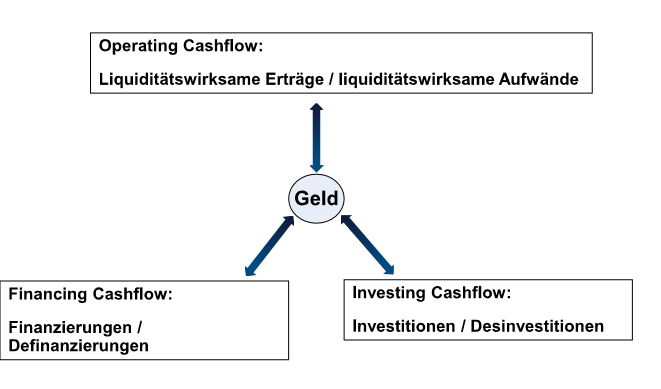
\includegraphics[width=0.3\textwidth]{Resources/Image/Cashflow.png}
\caption{\label{fig:Cashflow}Cashflow.}
\end{figure}

\subsubsection{Berechnung operativer Cashflow aus Erfolgsrechnung}
\begin{multicols}{2}
\begin{figure}[H]
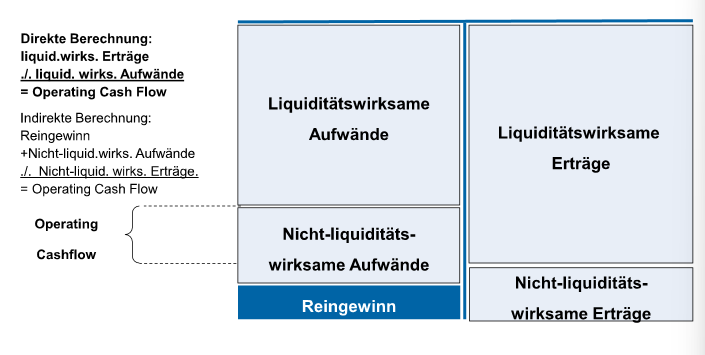
\includegraphics[width=0.3\textwidth]{Resources/Image/BerechnungCashflow.png}
\caption{\label{fig:BerechnungCashflow}BerechnungCashflow.}
\end{figure}

\columnbreak

\begin{figure}[H]
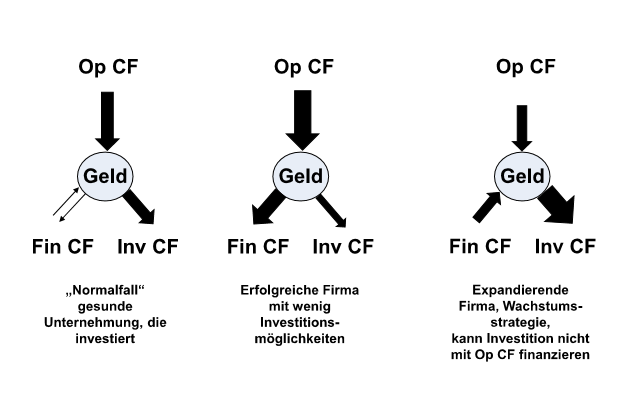
\includegraphics[width=0.3\textwidth]{Resources/Image/CashflowSchemata.png}
\caption{\label{fig:CashflowSchemata}CashflowSchemata.}
\end{figure}

\end{multicols}


\subsection{Hauptformen der Unternehmensfinanzierung}

\begin{figure}[H]
\centering
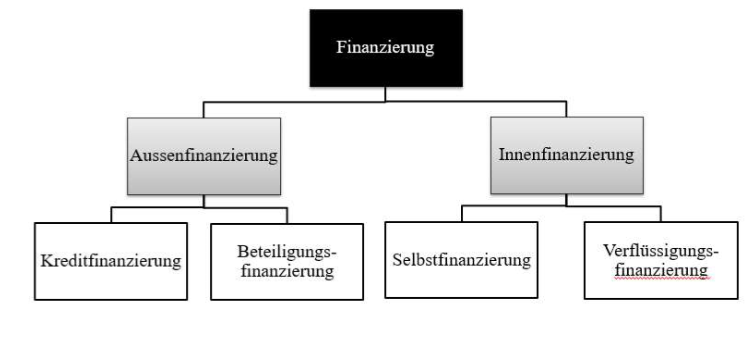
\includegraphics[width=0.3\textwidth]{Resources/Image/Unternehmensfinanzierung.png}
\caption{\label{fig:Unternehmensfinanzierung}Unternehmensfinanzierung.}
\end{figure}

\subsection{Rolle des CFO}

\paragraph{Management des Finanzdreiecks}

\begin{itemize}
	\item \colorbox{orange!30} {\textbf{Sicherheit}} (Sichere Anlagen ggf. weniger rentibel oder weniger liquid)
	\begin{itemize}
		\item Finanzielle Sicherheit, kein Konkursrisiko
	\end{itemize}
	\item \colorbox{orange!30} {\textbf{Rentabilität}} (Oft weniger sicher, oft langfristig gebunden)
	\begin{itemize}
		\item Sonst wird Verlust gemacht, Konkursgefahr!
	\end{itemize}
	\item \colorbox{orange!30} {\textbf{Liquidität}} (ggf.weniger sicher, können weniger rentabel sein)
	\begin{itemize}
		\item Auf Forderungen eingehen können (Zinsen, Steuern, Kosten, etc.)
	\end{itemize}
\end{itemize}

Stehen in einem Zielkonflikt, CFO muss sie in Einklang mit der Unternehmensstrategie bringen. So gestalten, dass unternehmerische Ziele erreicht werden.

\subsubsection{Kennzahlen}

\begin{table}[H]
\begin{tabular}{l|l|l}
\colorbox{blue!10}{\textbf{Kennzahl}} & \colorbox{blue!10}{\textbf{Formel}} & \colorbox{blue!10}{\textbf{Kommentar}} \\
\hline
\colorbox{teal!30} {\textbf{Liquidität}} \\
\hline
\textbf{Cash flow} & Geldzufluss - Geldabfluss aus Geschäftstätigkeit & sollte positiv sein\\
\hline
\textbf{Quick ratio} & (Zahlungsmittel + Debitoren) / \\& Kurzfristiges Fremdkapital & Können die kurzfristigen\\
&& Verpflichtungen erfüllt werden?\\
\hline
\colorbox{teal!30} {\textbf{Rentabilität}} \\
\hline
\textbf{Gesamtkapital-Rent}\\(ROI= Return of Investment) & EBIT / Gesamtkapital & Sollte höher als\\&& der FK-Zins sein\\
\hline
\textbf{Umsatz-Rent.}\\(ROS=Return of Sales) & Reingewinn / Umsatz \\
\hline
\textbf{Eigenkapital-Rent}\\(ROE=Return of Equity)& Reingewinn / Eigenkapital & Wichtig für Aktionäre\\
\hline
\colorbox{teal!30} {\textbf{Sicherheit}}\\
\hline
\textbf{Eigenfinanzierungsgrad} & Eigenkapital / Gesamtkapital & Mehr EK =\\&& Mehr Freiheitsgrade\\
\hline
\end{tabular}
\end{table}


\subparagraph{Hebel: Erhöhung der Gesamtkapitalrendite (ROI)\\}
= Rentabilitätsstrategie\\

Ertrag = Umsatzsteigerung\\
Aufwand = Operative Exzellenz\\
Anlagevermögen und Umlaufvermögen = Reduktion des investierten Kapitals\\

ROI = ((Ertrag - Aufwand)+ Fremdkapitalzinsen) / ((Anlagevermögen + Umlaufvermögen)+ Fremdkapital)\\
= EBIT  / Gesamtkapital


\subsubsection{ROE: Leverage Effect, Hebel für EK - Rendite}
$r_{G}$ = Gesamtkapitalrendite\\
i = interest (FK Zinssatz)\\
Bei Verlust wirkt Hebel in die andere Richtung!!!!\\
Der Leverage Effekt bzw. Verschuldungsgrad bringt hohes Risiko mit!!\\
\begin{figure}[H]
\centering
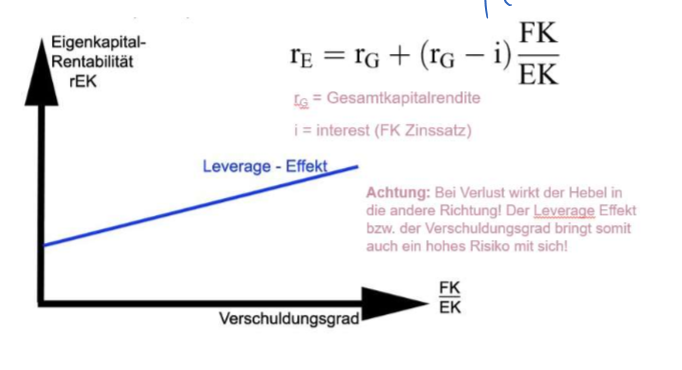
\includegraphics[width=0.3\textwidth]{Resources/Image/LeverageEffect.png}
\caption{\label{fig:LeverageEffect}LeverageEffect.}
\end{figure}



















\end{document}